%%%%%%%%%%%%%%%%%%%%%%%%%%%%%%%%%%%%%%%%%
% Cap\'itulo: Una teor\'ia de reescritura para SCCP (R) %
%%%%%%%%%%%%%%%%%%%%%%%%%%%%%%%%%%%%%%%%%
\chapter{Una teor\'ia de reescritura para SCCP (R)}
\label{chapter.rew}

Este cap\'itulo presenta una especificaci\'on formal del modelo \SCCP en la sintaxis de Maude~\cite{maude-book}. La especificaci\'on formal consta de un m\'odulo funcional que define el identificador de un agente; un m\'odulo funcional que define la sintaxis y los tipos requeridos para especificar los diferentes tipos de comandos u operadores disponibles en el modelo; y un m\'odulo funcional que define la sintaxis y los tipos requeridos para especificar los estados del modelo. Este m\'odulo incluye, entre otros, la definici\'on de un agente y un proceso. La transferencia de informaci\'on en \SCCP esta formalizada a partir de de reglas de reescritura que son parte de un m\'odulo de sistema.

Adicionalmente, este cap\'itulo presenta ejemplos de algunas simulaciones del modelo que usan la especificaci\'on formal y el comando \cde{rewrite} de Maude.

Las secciones~\ref{aid.rew},~\ref{syntax.rew} y~\ref{state.rew} presentan los m\'odulos funcionales \cde{AGENT-ID}, \cde{SCCP-SYNTAX} y \cde{SCCP-STATE}, respectivamente. La Secci\'on~\ref{rules.rew} presenta el modulo de sistema \cde{SCCP} que especifica las transiciones del modelo. Finalmente, la Secci\'on~\ref{example.rew} presenta algunos ejemplos de simulaci\'on del modelo usando el comando \cde{rewrite} de Maude.

%% Secci\'on: Especificaci\'on AGENT-ID%%
\section{Modelamiento formal del identificador}
\label{aid.rew}

El identificador de un agente est\'a representado por el sort \cde{Aid} definido en el modulo funcional \cde{AGENT-ID} de la siguiente manera:

\begin{maude}
  sort Aid .
  pr NAT .
  subsort Nat < Aid .

  op root : -> Aid .
  op _._ : Aid Aid -> Aid [assoc left id: root] .
\end{maude}

El identificador esta definido como una secuencia de n\'umeros naturales, representados por \cde{NAT}, concatenados con punto. La identidad izquierda de un identificador esta representada por \cde{root}, de forma que \cde{root.1} es equivalente a \cde{1}. Los n\'umeros de izquierda a derecha indican el espacio y subespacio al cual pertenece el agente, es decir, el identificador \cde{4.2.1} significa que el agente pertenece al espacio \cde{4}, dentro de este al subespacio \cde{2}, tal como se indica en la Figura~\ref{fig:agentid}.

\begin{figure}[htbp] %  figure placement: here, top, bottom, or page
   \centering
   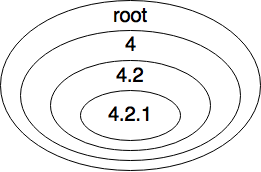
\includegraphics[width=2.5in]{idagent.png} 
   \caption{Identificador de un agente}
   \label{fig:agentid}
\end{figure}

%% Secci\'on:  %%
\section{Modelamiento formal de los operadores}
\label{syntax.rew}

Los operadores descritos en la Definici\'on~\ref{def:gensyn} est\'an representados por el sort \cde{SCCPCmd} en el modulo funcional \cde{SCCP-SYNTAX} tal como se muestra a continuaci\'on:

\begin{maude}
  sort SCCPCmd .

  op 0 : -> SCCPCmd . 
  op tell_ : Boolean -> SCCPCmd . 
  op ask_->_ : Boolean SCCPCmd -> SCCPCmd .
  op ask<_>_->_ : Aid Boolean SCCPCmd -> SCCPCmd .
  op _||_ : SCCPCmd SCCPCmd -> SCCPCmd [assoc gather (e E) ] .
  op <_>[_] : Aid SCCPCmd -> SCCPCmd .
\end{maude}

El argumento del operador $\textbf{tell(c)}$ es la restricci\'on o informaci\'on que se va a adicionar al banco de un agente, representado por un elemento de tipo \cde{Boolean}. El operador $\textbf{ask(c)} \rightarrow \textbf{P}$ tiene como argumentos la condici\'on a ser evaluada dentro del banco de informaci\'on del agente y el proceso a llevarse a cabo. Cada uno de estos argumentos esta representado por elementos del tipo \cde{Boolean} y \cde{SCCPCmd}, respectivamente.

%El proceso $P\|Q$ es para la ejecuci\'on en paralelo de procesos.
%El proceso $[P]_i$ ejecuta $P$ dentro del espacio de computaci\'on del agente $i$.

%% Secci\'on:  %%
\section{Modelamiento formal de agentes y procesos}
\label{state.rew}

\begin{maude}
fmod SCCP-STATE is
  pr SCCP-SYNTAX .
  pr SMT-UTIL .

  sorts Cid Obj Cnf Sys .
  subsorts Obj < Cnf .
  ops store process : -> Cid .
  op [_,_,_] : Cid Aid Boolean -> Obj [ctor] .
  op [_,_,_] : Cid Aid SCCPCmd -> Obj [ctor] .
  op mt : -> Cnf [ctor] .
  op __ : Cnf Cnf -> Cnf [ctor assoc comm id: mt] .
  op {_} : Cnf -> Sys [ctor] .

  vars L L0    : Aid .
  vars C C0    : Boolean .
  vars X       : Cnf .

  --- auxiliary operations
  op exists-store? : Cnf Aid -> Bool .
  eq exists-store?(mt, L)
   = false .
  eq exists-store?( [ process, L0, C0 ] X, L)
   = exists-store?(X,L) .
  eq exists-store?( [ store, L0, C0 ] X, L)
   = (L0 == L) or-else exists-store?(X,L) .
endfm
\end{maude}

%% Secci\'on:  %%
\section{Modelamiento formal de las transiciones}
\label{rules.rew}

present the transitions of the rewrite theory

\begin{maude}
--- non-observable concurrent transitions
  eq [ process, L, 0 ]
   = mt .
  eq [ store, L, B0 ] [ store, L, B1 ]
   = [ store, L, B0 and B1 ] .

  --- observable concurrent transitions
  rl [tell] :
     { [ store, L, B] [process, L, tell B0 ] X }
  => { [ process, L, 0 ] [ store, L, B and B0] X } .

 crl [ask] :
     { [ store, L, B ] [ process, L, ask B0  -> C0 ] X }
  => { [ store, L, B ] [ process, L, C0 ] X }
  if check-unsat(B and not(B0)) .

 crl [ask-ext0] :
     { [ store, L0 . L1, B ] [ process, L0, ask< L1 > B0  -> C0 ] X }
  => { [ store, L0 . L1, B ] [ process, L0, C0 ] X }
  if check-unsat(B and not(B0)) . 

 crl [ext-ask1] :
     { [ process, L0, ask< L1 > B0  -> C0 ] X }
  => { [ process, L0, C0 ] X }
  if exists-store?(X, L0 . L1) == false
  /\ check-unsat(not(B0)) . 

  rl [parallel] :
     { [ process, L, C0 || C1 ] X }
  => { [ process, L, 0 ] [ process, L, C0 ] [ process, L, C1 ] X } .

  rl [space] :
     { [ process, L0, < L1 >[ C0 ] ] X } 
  => { [ process, L0, 0 ] [ process, L0 . L1, C0] [ store, L0 . L1, true ] X } .
\end{maude}

%% Secci\'on:  %%
\section{Ejemplos}
\label{example.rew}


